 \PassOptionsToPackage{unicode}{hyperref}
\PassOptionsToPackage{hyphens}{url}
%
\documentclass[12pt, a4paper]{article}
\usepackage[a4paper,margin=1in]{geometry}
\setlength\parindent{0pt}
\usepackage{mathptmx}
\usepackage{amsmath,amssymb}
\usepackage[T1]{fontenc}
\usepackage[utf8]{inputenc}
\usepackage{textcomp}
\usepackage{float}
\usepackage{graphicx}
\usepackage{caption}
\usepackage{subcaption}

\author{Jaspinder Singh, Artificial Intelligence, 0001138673 
\\Othmane Darbouri, Artificial Intelligence, 0001145623
\\Anastasia Valevich, Artificial Intelligence, 0001113159
\\Hilina Fissha Woreta, Artificial Intelligence, 0001143250 }
\date{}
\title{Social Network Analysis of "Game of Thrones" series}

\begin{document}
\maketitle

\section{Introduction}

\label{introduction}
Literature, a rich domain reflecting human complexities, encompasses diverse genres and formats. Fantasy literature, in particular, stands out for its intricate worlds and complex characters. While poetry is often celebrated as a pinnacle of literary expression, narrative prose, especially novels, offers immersive journeys through human experiences. This project focuses on fantasy novels, specifically George R.R. Martin's A Song of Ice and Fire series, famously known as Game of Thrones.
\\\\Through the lens of social network analysis, this study examines the intricate web of character interactions that define this epic saga, merging literature with network analysis to explore its narrative structure and complex character dynamics. The series, a landmark in fantasy literature, portrays the struggle for power across Westeros and Essos, with noble families vying for the Iron Throne amid alliances and betrayals. Key characters like Eddard Stark, Daenerys Targaryen, and Tyrion Lannister play pivotal roles in shaping the plot.
\\\\In this project, we undertake a comprehensive analysis of these character interactions, using social network analysis techniques to map and quantify relationships. This approach enables us to trace the evolution of key relationships and identify influential characters across the series. By exploring "Game of Thrones" through this analytical perspective, we aim to deepen our understanding of the saga's narrative structure and uncover patterns that may not be immediately visible, adding a new dimension to the literary analysis of this iconic series.

\section{Problem and Motivation}
\label{problem-and-motivation}
This project conducts a social network analysis of George R.R. Martin’s Game of Thrones series, focusing on the complex relationships and evolving dynamics between characters. By analyzing alliances, enmities, and shifting power structures, the study aims to provide deeper insights into the series’ intricate narrative.
\\\\One of the primary objectives of this analysis is to identify the main characters by calculating centrality measures within the character network. These metrics provide insights into character prominence and significance within the story, allowing us to assess the roles each character plays at the plot level.
\\\\In addition, this analysis seeks to uncover character groups or clusters within the network. Identifying such clusters serves two purposes: it sheds light on alliances and conflicts that drive the narrative, and it allows for a comparison of these analytical findings with known alliances in the story. If the clusters identified in the network align with known group dynamics in the series, this can enhance confidence in the dataset’s validity and the accuracy of the social network model.
\\\\Theoretical importance also underlies this project, as studying fictional social networks offers a controlled environment for exploring the evolution of complex character relationships. This work further demonstrates the applicability of social network analysis to literary studies, revealing plot insights that may not be apparent through traditional analysis methods.

\section{Datasets}
\label{datasets}
The Game of Thrones Online Dataset is a free, publicly available dataset published on the Kaggle online platform. The dataset contains all the characters in the story set out in the books of the Song of Ice and Fire cycle, and is designed to reflect all the interactions of the characters throughout the five books.
\\\\The data was collected by searching for the names of the characters: two characters are considered to co-occur if their names appear in the vicinity of 15 words from one another in the books.
\\\\This dataset is a network and is presented as a text file describing the boundaries between characters, with some attributes attached to each boundary. There are 5 corresponding columns in the dataset: Source, Target, Type, Weight, and Book. The Source and the Target are two nodes that are connected by an edge. A network can have directional or non-directional edges, in this network all edges are non-directional.
\\\\As soon as the name (Source) occurs, the number of interactions (Weight) with other names (Target) in a specific part of the books (Book) is located at the distance of the next 15 words. The interactions are calculated in such a way that if a new name were specified in these 15 words, a connection with a weight equal to 1 would appear between the two nodes. If an edge already exists, +1 is added to the edge weight.
\\\\There are no cases in the dataset when Source and Target replace each other and have different numbers of interactions, i.e. we do not have the following problem:
\\\textit{Source = Addam-Marbrand, Target = Jaime-Lannister, Book = 1, Weight = 3}
\\\textit{Source = Jaime-Lannister, Target = Addam-Marbrand, Book = 1, Weight = 5}
\\Therefore, all edges are undirected.
\\\\Network X was used to implement the network structure and subsequent analysis [4]. As a result, 5 different networks were obtained, each of which corresponds to one of the 5 books. All networks are weighted and undirected graphs. Each node corresponds to one character, and the presence of an edge between two nodes reflects the interaction between two characters. There are neither proper edges nor multiple edges.
\\\\It was decided that the graph, which includes all 5 books, will also be studied. A total of 796 vertices and 2822 edges were found. Table 1 shows the distribution of these vertices and arcs between the books.

\begin{table}[H]
    \centering
    \begin{tabular}{c|c|c|c|c|c|c}
    \hline
         & Book1 & Book2 & Book3 & Book4 & Book5 & All Books\\
        Nodes & 187 & 266 & 293 & 309 & 325 & 796\\
        Edges & 684 & 774 & 1008 & 682 & 760 & 2822\\
    \hline
    \end{tabular}
    \caption{Table 1: Number of nodes and edges for each book}
    \label{tab:my_label}
\end{table}

\begin{figure}[H]
\centering
\begin{subfigure}{.5\textwidth}
  \centering
  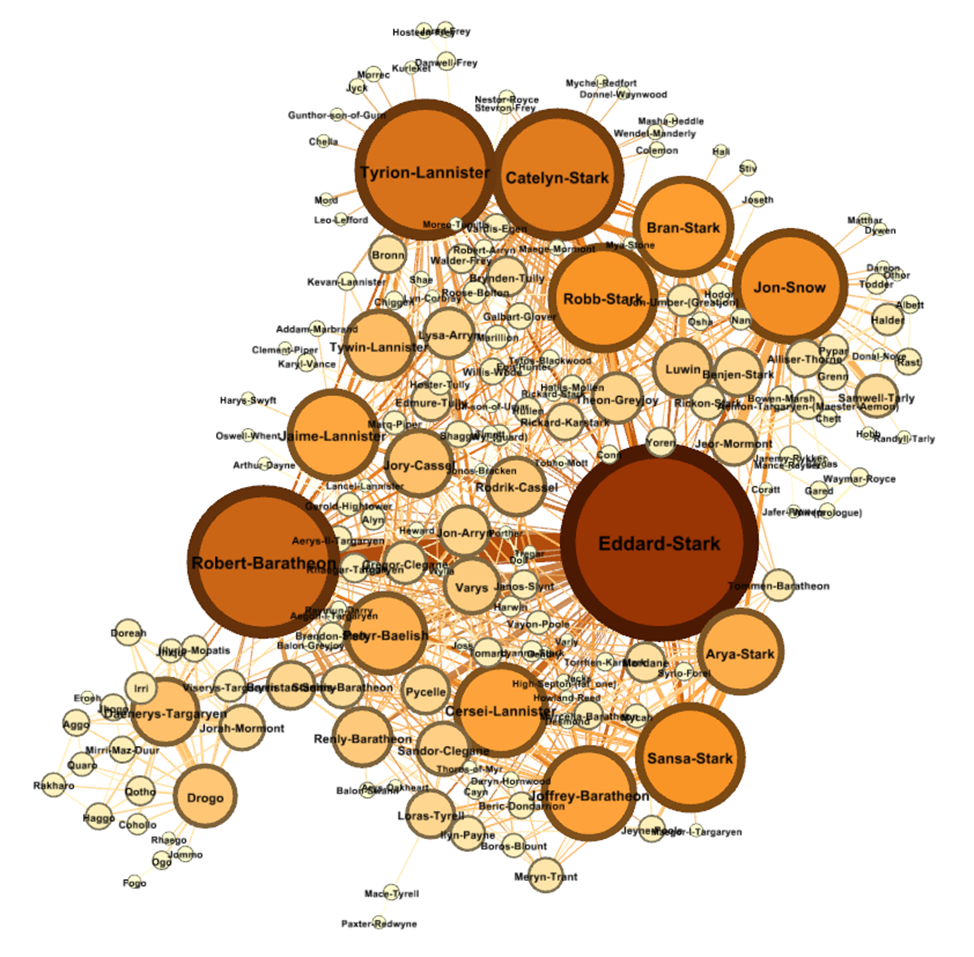
\includegraphics[width=1\linewidth]{book_1.png}
  \caption{Book 1}
  \label{fig:sub1}
\end{subfigure}%
\begin{subfigure}{.5\textwidth}
  \centering
  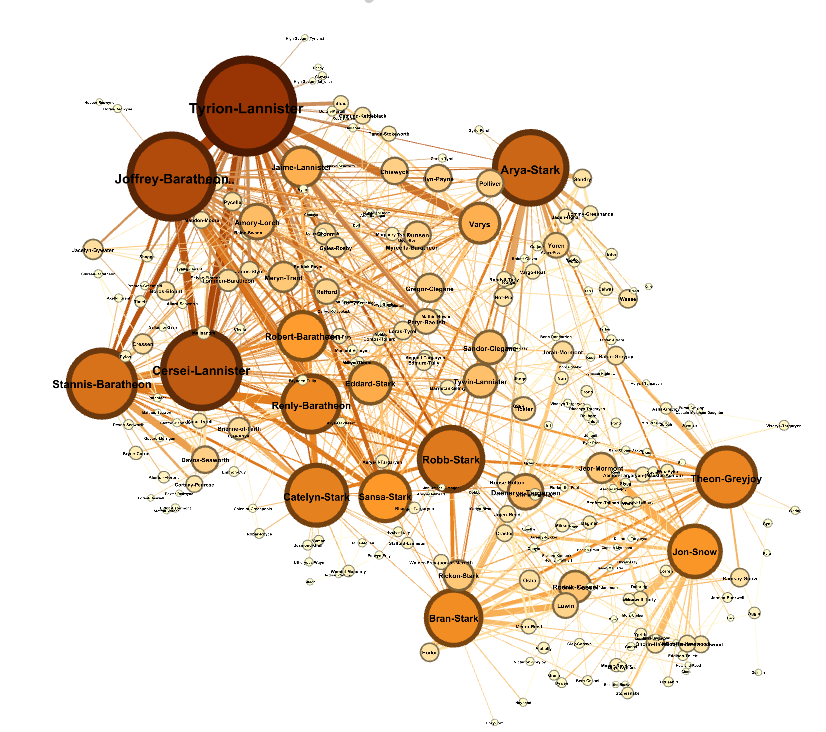
\includegraphics[width=1\linewidth]{book_2.png}
  \caption{Book 2}
  \label{fig:sub2}
\end{subfigure}
\caption{Graphs from Book 1 and Book 2. Nodes dimensions depend on their degree.}
\label{fig:test}
\end{figure}

\section{Validity and Reliability}
\label{validity-and-reliability-not-needed-for-the-project-proposal}
Validity reflects how well the dataset captures the fictional reality of the Game of Thrones universe. Since it was compiled by a Kaggle user, its validity cannot be guaranteed with absolute certainty. This is further influenced by the subjective interpretation of what qualifies as an "interaction" between characters—for example, the assumption that two names appearing within 15 words of each other indicate interaction may not always hold true.
\\\\The reliability of the data set is confirmed by two factors. First, the fact that the dataset is hosted on a platform recognized for its reliable and expert-verified datasets assumes a reasonable level of accuracy. Secondly, the dataset has a bronze medal on the platform. Such medals are awarded to popular publicly available datasets. Authors' own votes and the votes of newcomers are not taken into account when counting medals.
\\\\The reliability of the dataset can be deemed high, as it originates from a publicly accessible database hosted on Kaggle, which is well-organized and easy to download. By adhering to standard data pre-processing procedures, the study can be easily reproduced by other researchers using the same dataset.

\section{Measures and Results}
\label{measures}
\subsection{Degree Centrality}
\label{degree centrality}
Our first aim was to understand which nodes were the ones with larger degree centrality in each book (i.e. main characters). An example of the values we obtained is reported in Fig. 2, where Eddard-Stark stands out above all the others, as expected. To find other main characters, we set a threshold for significance in each book. We decided to use a threshold of 0.20 to find the following main characters: Eddard Stark, Robert Baratheon, Tyrion Lannister, Catelyn Stark. This is true both for the first book and for all books taken together.

\begin{figure}[H]
    \centering
    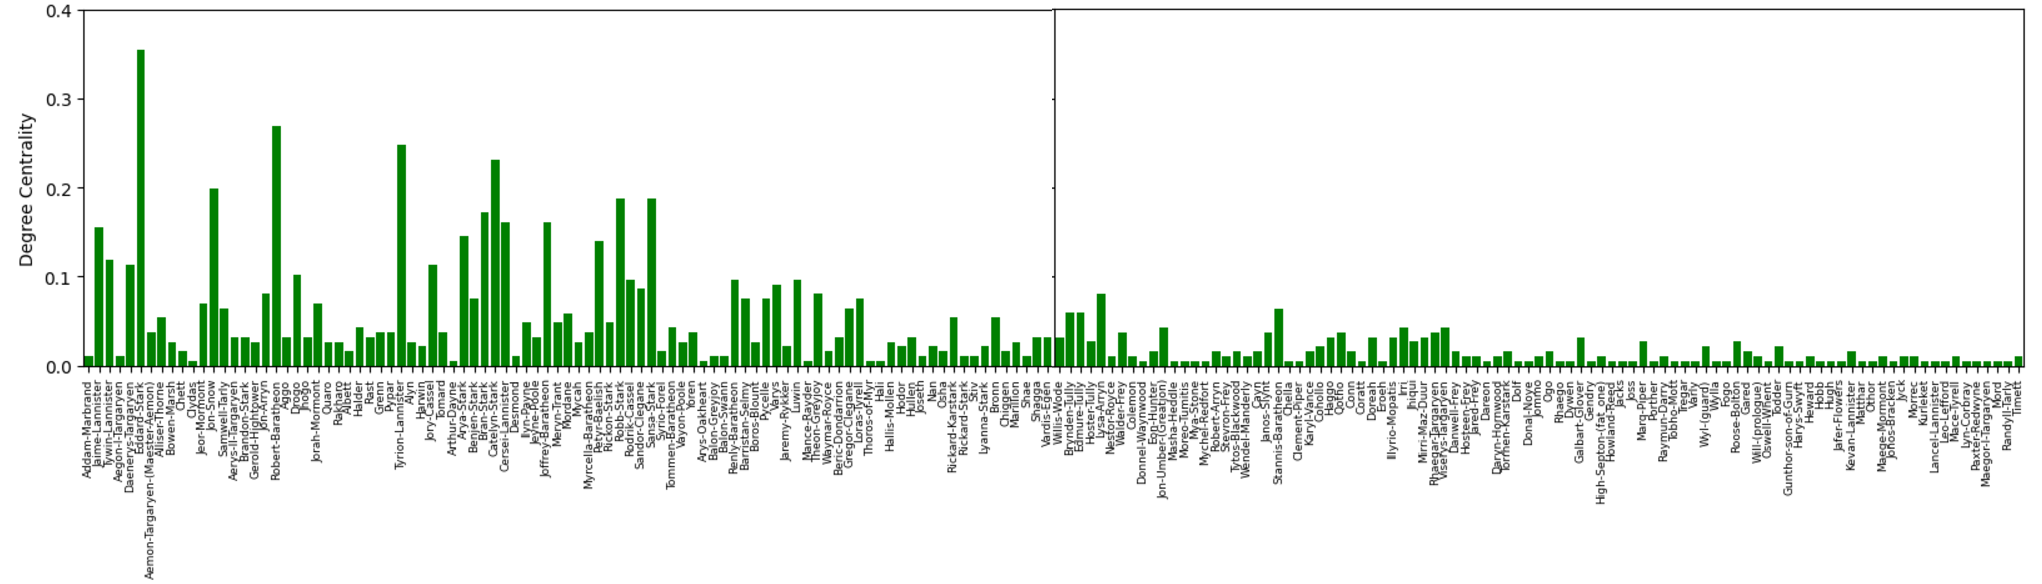
\includegraphics[width=1\linewidth]{book_1_main_character.png}
    \caption{Histogram of degree centrality values for each node in Book 1.}
    \label{fig:enter-label}
\end{figure}

To test scale invariance, we plotted the value distribution on a log-log scale and performed a linear regression, excluding Eddard Stark as an outlier due to his disproportionately high centrality. Figure 3 illustrates the linear fit for Book 1.

\begin{figure}[H]
    \centering
    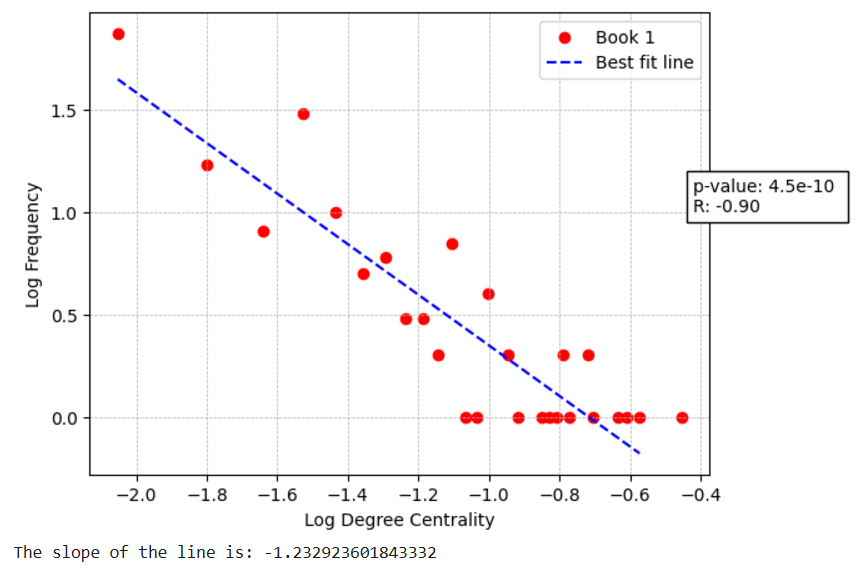
\includegraphics[width=0.5\linewidth]{Log-log plot of the degree distribution for Book 1.png}
    \caption{Log-log plot of the degree distribution for Book 1.}
    \label{fig:enter-label}
\end{figure}

The cumulative distribution of centrality scores for both the first book and the overall graph was also computed (as shown in Figure 4). The resulting graph is a stepwise increasing curve, which is clearly visible on a logarithmic scale. This is expected, as the degrees are normalized and calculated as ratios of integers, leading to discrete values. Consequently, as the values increase along the x-axis, the total value initially remains constant for absent values, followed by a sharp rise when discrete values become available.

\begin{figure}[H]
    \centering
    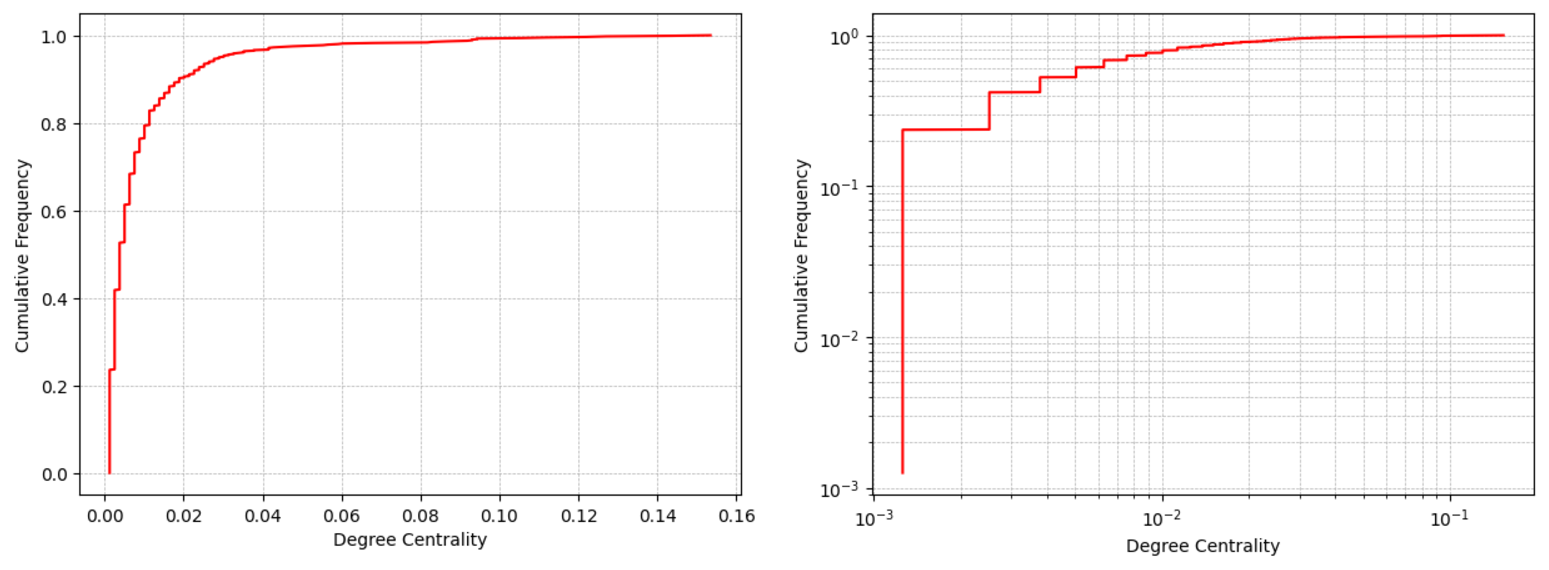
\includegraphics[width=1\linewidth]{Cumulative distribution of degree centrality.png}
    \caption{Cumulative distribution of degree centrality on both a normal scale and a logarithmic plot for the entire network.}
    \label{fig:enter-label}
\end{figure}

\subsection{Eigenvector Centrality}
\label{eigenvector centrality}
Eigenvector centrality offers an alternative method for identifying key characters by assigning greater significance to nodes connected to other influential nodes. The results from this measure differ from those of degree centrality, as seen qualitatively in Figure 5. Using eigenvector centrality, certain nodes gain additional prominence, while others lose it.

\begin{figure}[H]
    \centering
    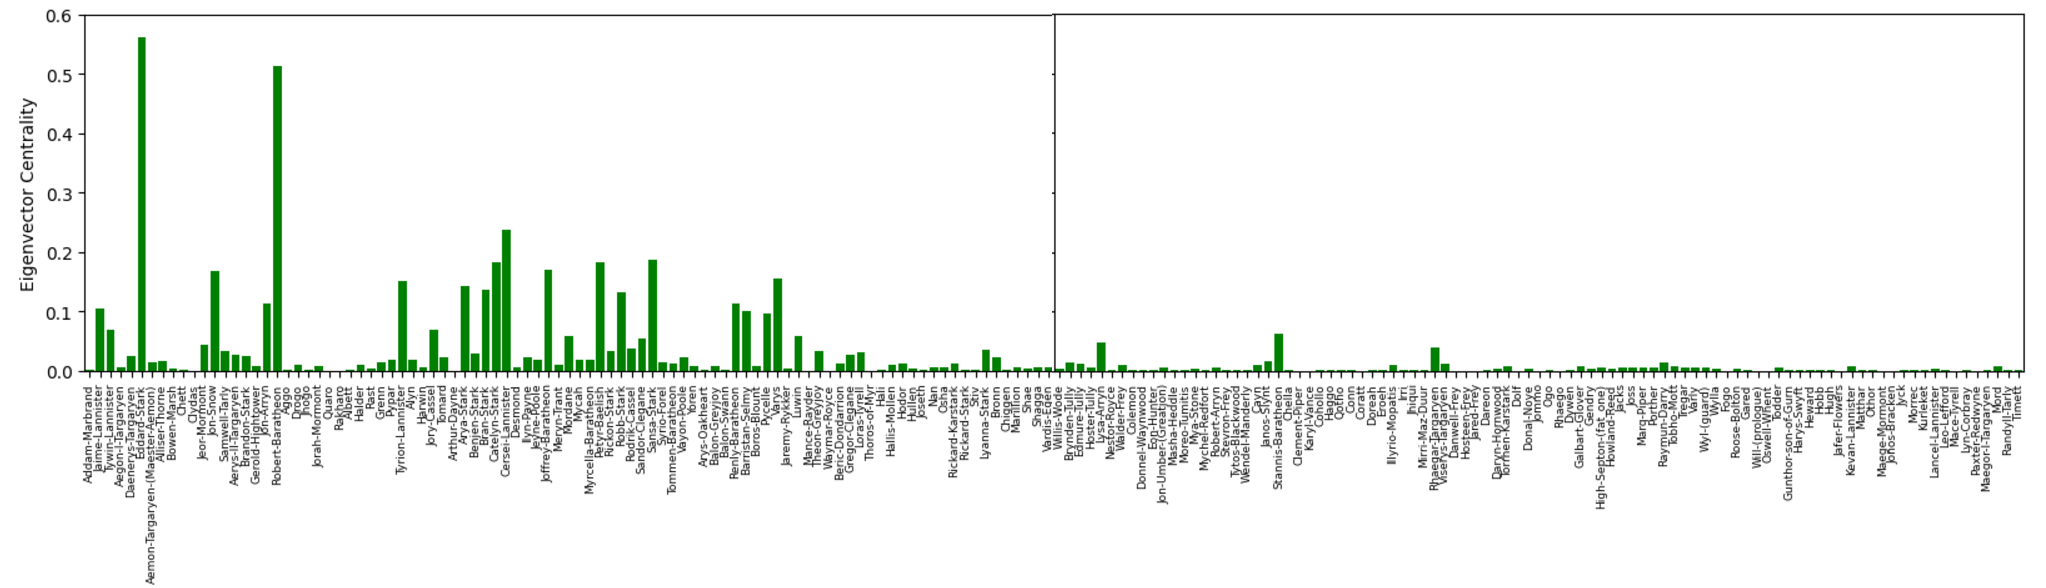
\includegraphics[width=1\linewidth]{Eigenvector centrality values of nodes in Book 1.png}
    \caption{Eigenvector centrality values of nodes in Book 1.}
    \label{fig:enter-label}
\end{figure}

More specifically, using the same threshold as before, we found the following characters: Eddard-Stark, Robert-Baratheon, Cersei-Lannister. It can be seen that Eddard-Stark and Robert-Baratheon have become more significant. Tyrion Lannister and Catelyn Stark have lost their importance significantly. Finally, we can observe how Cersei-Lannister has become "important", although its importance has increased only slightly. It's just that the other figures in the book have lost their importance.
\\\\Figure 6 presents the eigenvector centrality distribution as a scatter plot, along with its cumulative value on a logarithmic scale for Book 1. Visually, the scatter plot appears to be right-skewed, while the cumulative distribution forms a straight line, as anticipated.

\begin{figure}[H]
    \centering
    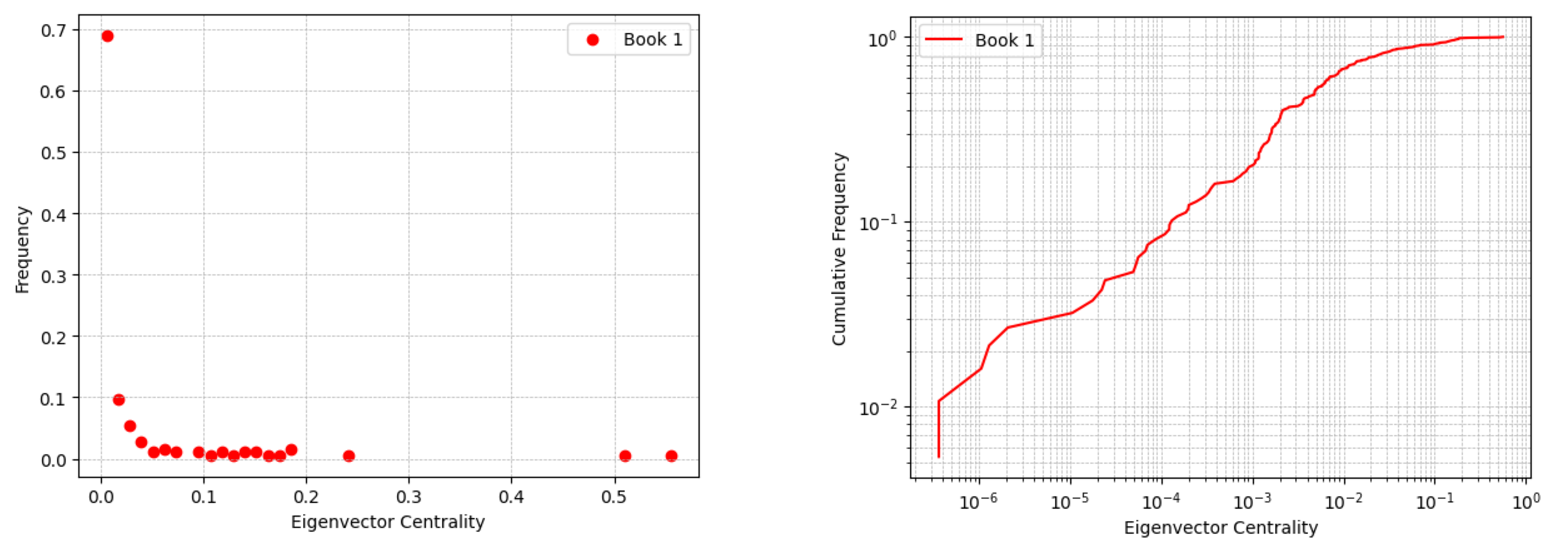
\includegraphics[width=1\linewidth]{Eigenvector centrality distribution and Cumulative Distribution for Eigenvector Centrality.png}
    \caption{Eigenvector centrality distribution and Cumulative Distribution for Eigenvector Centrality.}
    \label{fig:enter-label}
\end{figure}

\subsection{Betweenness Centrality}
\label{betweenness centrality}
To identify nodes acting as "bridges" in interactions, we calculated the betweenness centrality. The majority of nodes were found to have scores close to zero, indicating they lie outside the main shortest paths in the graphs. For instance, the results for Book 1 are displayed in Figure 7.

\begin{figure}[H]
    \centering
    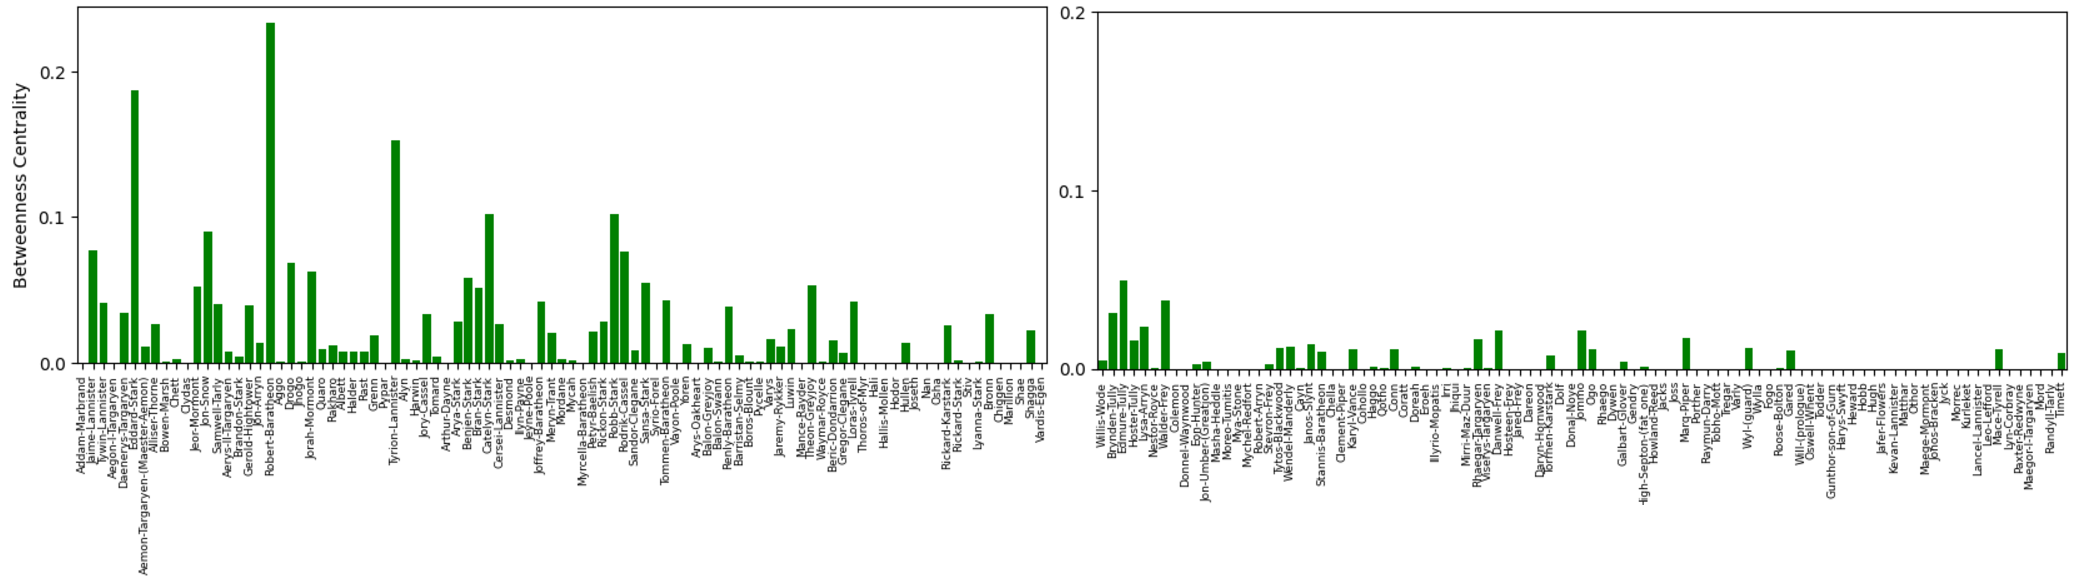
\includegraphics[width=1\linewidth]{Betweenness centrality.png}
    \caption{Betweenness centrality values for nodes in Book 1, with most nodes having scores of zero or close to zero.}
    \label{fig:enter-label}
\end{figure}

In the first book and in all the books combined the node with betweenness centrality above a certain threshold is Robert-Baratheon. Some characters disappeared. This shows how different centrality measures characterize the importance of the characters in different ways.

\subsection{Closeness centrality}
\label{closeness centrality}
As expected, Eddard-Stark and Robert-Baratheon were found to have the largest closeness centrality values in all the networks (e.g. nearly 0.56 and 0.54 in book 1, Fig. 8). This means that they is maximally close to most of the nodes in the network.

\begin{figure}[H]
    \centering
    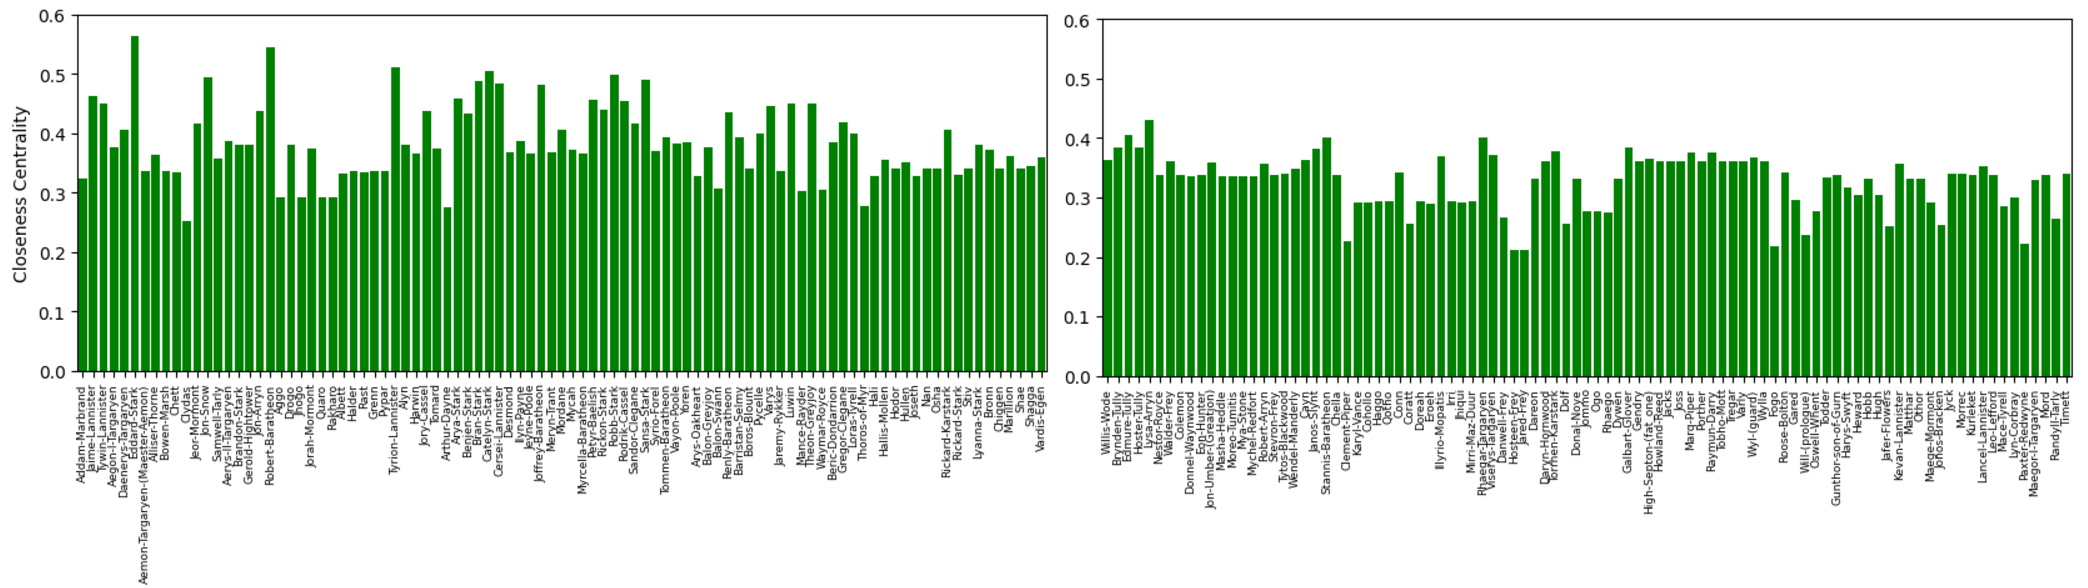
\includegraphics[width=1\linewidth]{Closeness centrality values of nodes in book 1..png}
    \caption{Closeness centrality values of nodes in Book 1.}
    \label{fig:enter-label}
\end{figure}
\subsection{Local Clustering coefficient}
In network analysis, the local clustering coefficient quantifies how close a node's neighbors are to being a complete graph. In Book 1, our analysis shows that central characters like Eddard Stark and Robert Baratheon demonstrate high clustering coefficients (>0.8), indicating their position within tightly-knit communities. Characters like Tyrion Lannister and Catelyn Stark show medium clustering values (0.4-0.7), reflecting their roles as bridges between different social groups. Notably, characters such as Varys and Petyr Baelish exhibit low clustering coefficients (<0.3), aligning with their roles as information brokers maintaining deliberately sparse connections.

\begin{figure}[H]
    \centering
    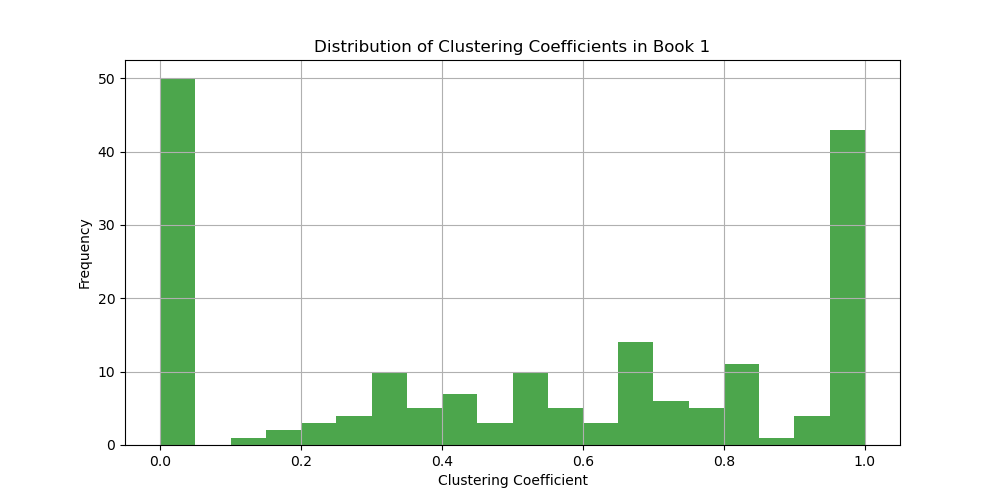
\includegraphics[width=1\linewidth]{clustering_book1.png}
    \caption{Distribution of Clustering Coefficients in Book 1, showing character interaction patterns}
    \label{fig:clustering}
\end{figure}

\subsection{Cliques}
The analysis of cliques reveals key character groups within the narrative. In Book 1, the most prominent clique centers around the King's Landing court, including Eddard Stark, Robert Baratheon, and the Lannisters. Another significant clique forms around Winterfell, comprising the Stark family members. These cliques effectively capture the major centers of power and influence in the early narrative, particularly showing how the story revolves around interactions between noble houses.

\begin{figure}[H]
    \centering
    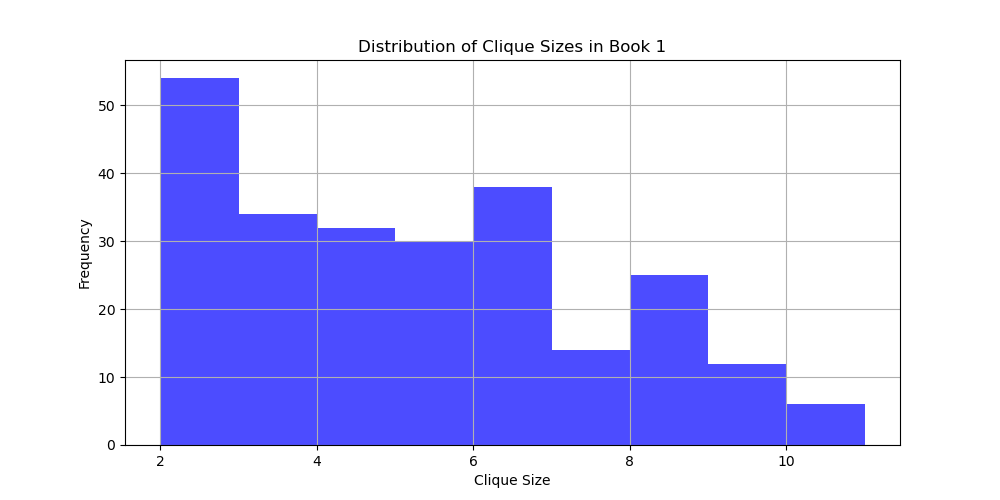
\includegraphics[width=1\linewidth]{cliques_book1.png}
    \caption{Distribution of Clique Sizes in Book 1, showing character group formations}
    \label{fig:cliques}
\end{figure}

\subsection{K core and core periphery structures}
The k-core decomposition reveals the hierarchical structure of character interactions. The highest k-core (k=9) contains central figures like Eddard Stark and Robert Baratheon, while lower cores include secondary characters like household members and guards. This structure reflects the narrative's organization, with character importance diminishing as k-value decreases, matching their roles in the story's development.

\begin{figure}[H]
    \centering
    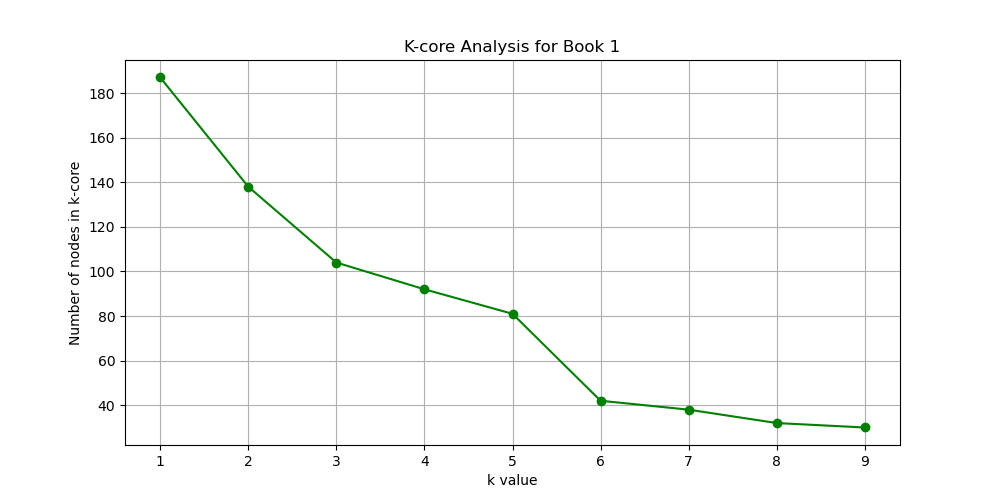
\includegraphics[width=1\linewidth]{kcore_book1.png}
    \caption{K-core Analysis for Book 1, showing character importance levels}
    \label{fig:kcore}
\end{figure}

\subsection{Density}
Network density across the five books quantifies the story's expanding scope. Book 1 shows the highest density (0.039), centered on narratives in King's Landing and Winterfell. The density decreases through subsequent books, reaching its lowest in Book 5 (0.015), reflecting the story's evolution from a focused political conflict into a sprawling epic spanning multiple continents and plotlines.

\begin{figure}[H]
    \centering
    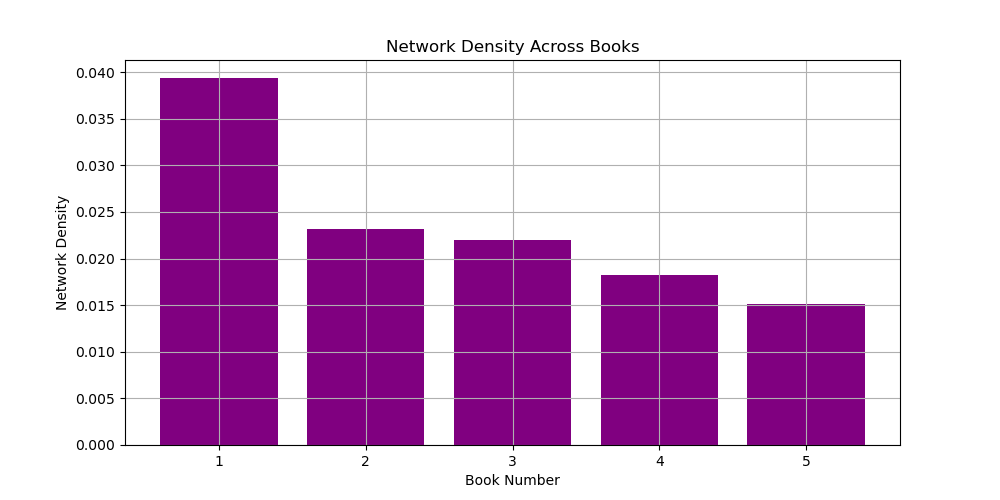
\includegraphics[width=0.8\linewidth]{density_books.png}
    \caption{Network Density Across Books, showing narrative expansion}
    \label{fig:density}
\end{figure}
\section{Conclusion}
Through our network analysis journey of Game of Thrones, we've uncovered the intricate ways George R.R. Martin builds his world of ice and fire. By examining character importance through various lenses, a fascinating story emerges. Initially, we see Eddard Stark and Robert Baratheon dominating the network as central figures, while characters like Littlefinger operate from the shadows, showing lower centrality but crucial bridging roles. The tight-knit communities of Winterfell and King's Landing appear as dense clusters in our early analysis, reflecting the concentrated power centers of Westeros.

What's particularly captivating is how our measurements capture the story's grand evolution. The steady decline in network density from Book 1 to Book 5 mathematically mirrors what readers experience - the transformation from an intimate political drama to a sprawling epic. Our k-core analysis reveals the hierarchical nature of Martin's world, while the negative assortative mixing beautifully captures Westeros's rigid social ladder, where high-born characters primarily interact with their subordinates. Through these various metrics, we've quantified not just how characters connect, but how Martin masterfully expands his narrative while maintaining its intricate social web.

\section{Critique}
Looking back at our analytical journey, we see both achievements and missed opportunities. While we successfully mapped out the network's evolution and character relationships, we feel there's more to the story we could have uncovered. Think of our 15-word proximity measure like trying to understand friendships by only counting when people stand near each other - it tells us something useful, but misses the rich complexity of real relationships. 

We could have enriched our analysis by considering the emotional weight of character interactions - after all, not all conversations in Game of Thrones carry equal significance. Some of the most pivotal moments in the series might be brief exchanges with profound implications. Adding geographic information could have helped us better understand how physical distances influence the story's network structure, especially as characters embark on their separate journeys. While our current analysis gives us a solid foundation for understanding Martin's complex world, these additions would have helped us tell an even richer story about how his characters connect, clash, and evolve throughout the series.
\end{document}
